\section{Etherless-server}
	\subsection{Overview} % Descrizione dell'architettura utilizzata, compresi i design pattern
	Etherless-server is the module that listens to events emitted by the Etherless-smart module and processes them through chosen operations. In order to implement these functionalities, the following architecture was designed and developed.
	\subsection{Architecture}
	\subsubsection{EventsManagement}
	This package manages the listening of events and controls their processing.
	\begin{figure} [h!]
		\centering
		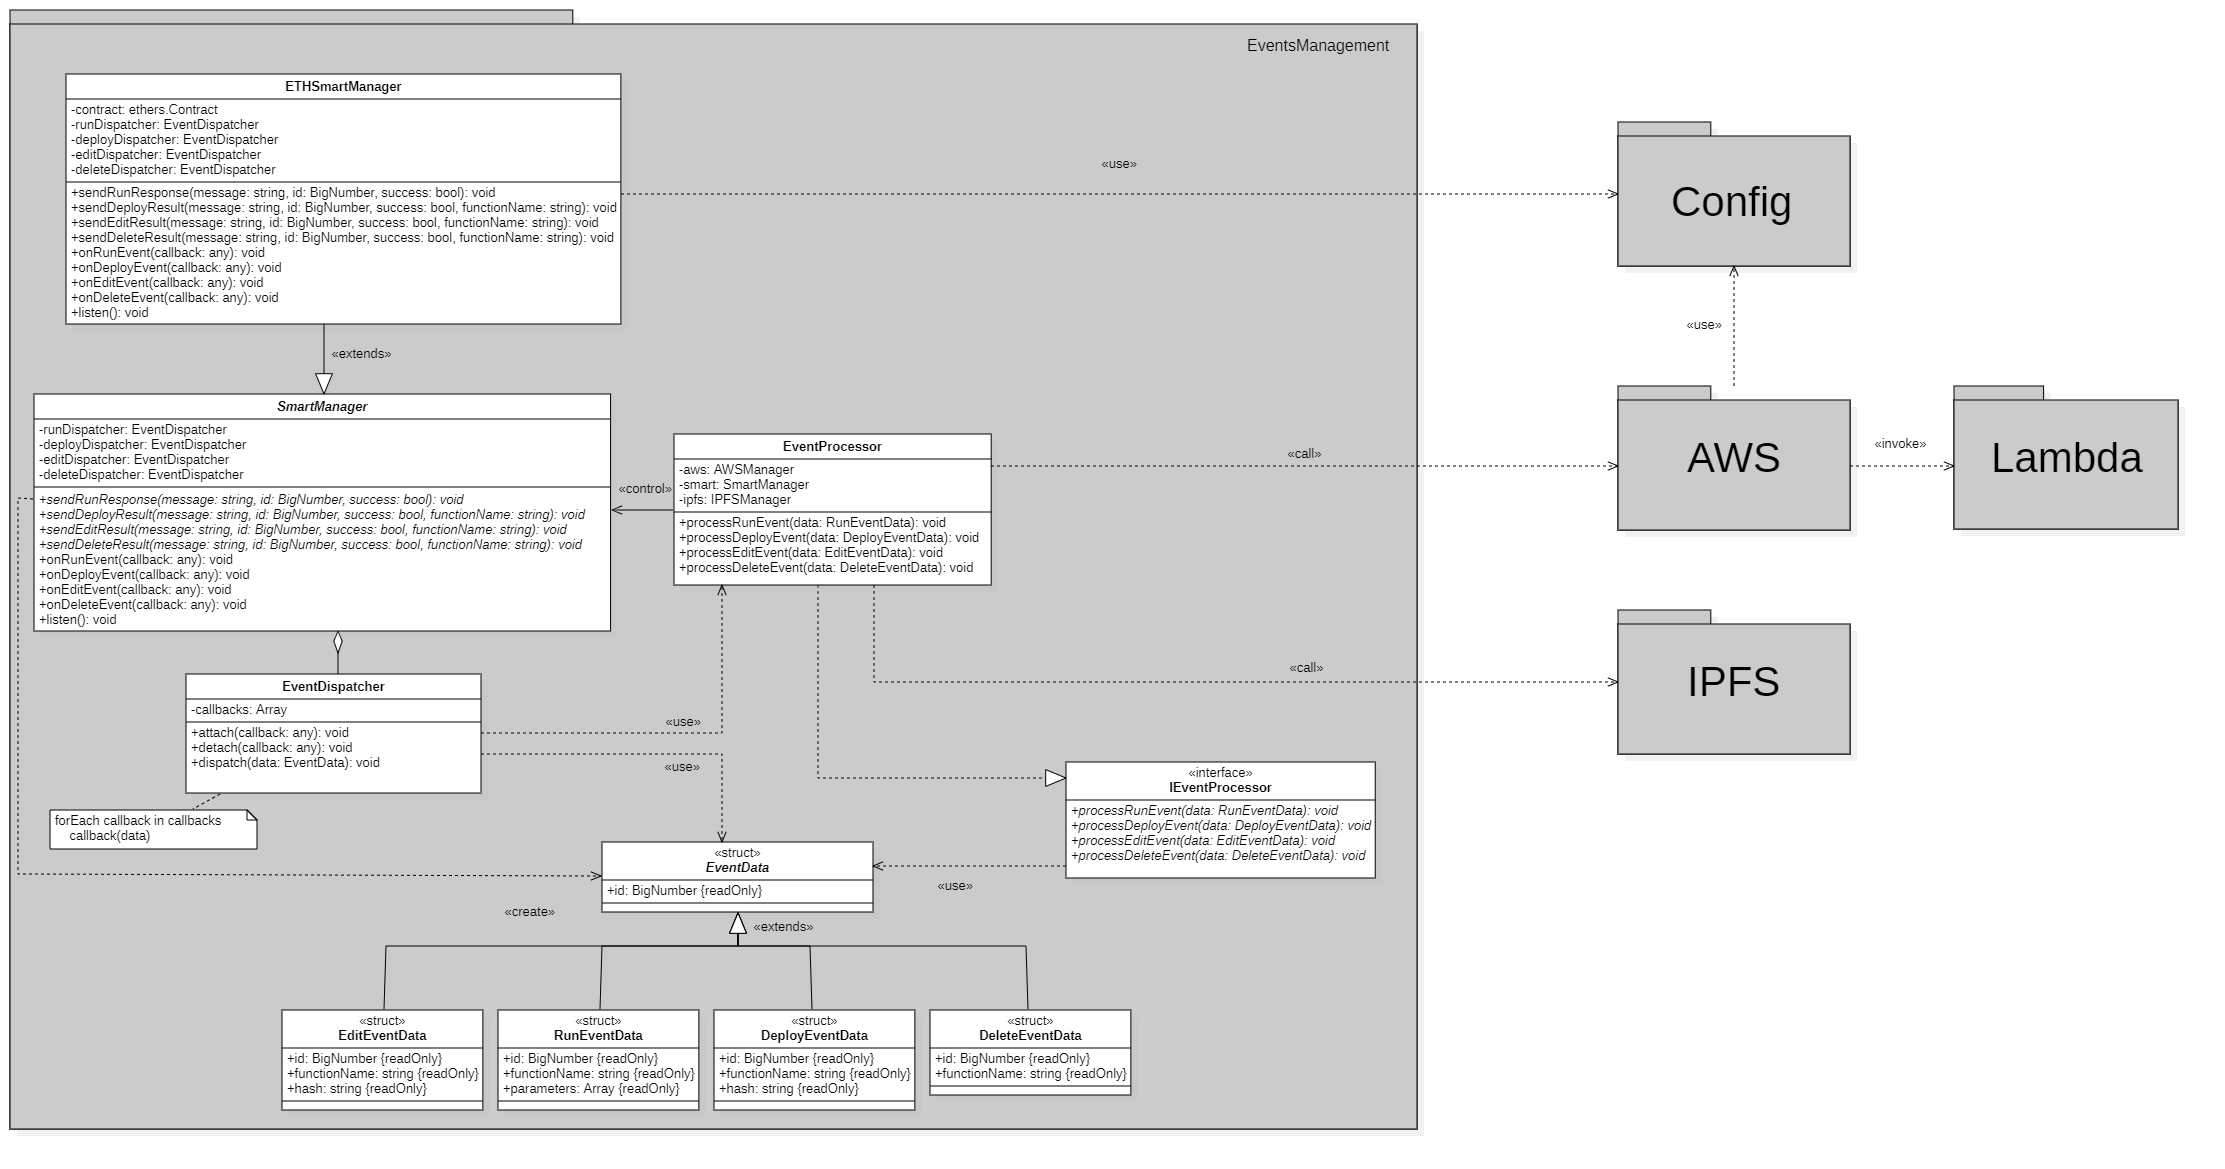
\includegraphics[width=1.1\linewidth]{diagrammi/etherless-server/Eventsmanager}
		\caption{Class diagram of the EventsManagement package.}
	\end{figure}
	\subsubsubsection{EventDispatcher}
	Class which forwards a given EventData object to all the objects that have subscribed to it. An object can subscribe to an EventDispatcher through its \texttt{attach} method, specifying a callback to be called with the EventData as parameter.
	\subsubsubsection*{Attributes}
	\begin{itemize}
		\item \textbf{callbacks}: array containing all the callbacks to be run when the \texttt{dispatch} method is called.
	\end{itemize}
	\subsubsubsection*{Methods}
	\begin{itemize}
		\item \textbf{attach}: inserts a new callback in the callbacks array;
		\item \textbf{detach}: removes a callback from the callbacks array;
		\item \textbf{dispatch}: forwards a given EventData to all the objects that have subscribed to it, through the invocation of the callbacks provided in the callbacks array.
	\end{itemize}
	\subsubsubsection{SmartManager}
	Abstract class whose derivatives allow to listen to external events, create processing requests and send responses to the external events source.
	\subsubsubsection*{Attributes}
	\begin{itemize}
		\item \textbf{runEventDispatcher}: EventDispatcher object, used to dispatch run processing requests represented by RunEventData objects;
		\item \textbf{deployEventDispatcher}: EventDispatcher object, used to dispatch deploy processing requests represented by DeployEventData objects;
		\item \textbf{editEventDispatcher}: EventDispatcher object, used to dispatch edit processing requests represented by EditEventData objects;
		\item \textbf{deleteEventDispatcher}: EventDispatcher object, used to dispatch delete processing requests represented by DeleteEventData objects;
	\end{itemize}
	\subsubsubsection*{Methods}
	\begin{itemize}
		\item \textbf{sendRunResult}: sends the result of a previously received run request back to the event source. The response contains a message and useful request related information.
		\item \textbf{sendDeployResult}: sends the result of a previously received deploy request back to the event source. The response contains a message and useful request related information.
		\item \textbf{sendEditResult}: sends the result of a previously received edit request back to the event source. The response contains a message and useful request related information.
		\item \textbf{sendDeleteResult}: sends the result of a previously received delete request back to the event source. The response contains a message and useful request related information;
		\item \textbf{onRun}: allows to subscribe a callback to the runEventDispatcher attribute;
		\item \textbf{onDeploy}: allows to subscribe a callback to the deployEventDispatcher attribute;
		\item \textbf{onEdit}: allows to subscribe a callback to the editEventDispatcher attribute;
		\item \textbf{onDelete}: allows to subscribe a callback to the deleteEventDispatcher attribute;
		\item \textbf{dispatchRunEvent}: runs all callbacks in the runEventDispatcher callbacks array with data as parameter;
		\item \textbf{dispatchDeployEvent}: runs all callbacks in the deployEventDispatcher callbacks array with data as parameter;
		\item \textbf{dispatchEditEvent}: runs all callbacks in the editEventDispatcher callbacks array with data as parameter;
		\item \textbf{dispatchDeleteEvent}: runs all callbacks in the deleteEventDispatcher callbacks array with data as parameter.
	\end{itemize}
	\subsubsubsection{ETHSmartManager}
	Class derived from SmartManager, which acts as an Ethereum events listener.
	\subsubsubsection*{Attributes}
	\begin{itemize}
		\item \textbf{contract}: instance of an Ethereum smart contract used to listen to Ethereum events and communicate with the smart contract itself;
		\item \textbf{runEventDispatcher}: EventDispatcher object used to dispatch run processing requests represented by RunEventData objects;
		\item \textbf{deployEventDispatcher}: EventDispatcher object used to dispatch deploy processing requests represented by DeployEventData objects;
		\item \textbf{editEventDispatcher}: EventDispatcher object used to dispatch edit processing requests represented by EditEventData objects;
		\item \textbf{deleteEventDispatcher}: EventDispatcher object used to dispatch delete processing requests represented by DeleteEventData objects;
	\end{itemize}
	\subsubsubsection*{Methods}
	\begin{itemize}
		\item \textbf{sendRunResult}: sends the result of a previously received run request back to Etherless-smart. The response contains a message and useful request related information.
		\item \textbf{sendDeployResult}: sends the result of a previously received deploy request back to Etherless-smart. The response contains a message and useful request related information.
		\item \textbf{sendEditResult}: sends the result of a previously received edit request back to Etherless-smart. The response contains a message and useful request related information.
		\item \textbf{sendDeleteResult}: sends the result of a previously received delete request back to Etherless-smart. The response contains a message and useful request related information;
		\item \textbf{onRun}: allows to subscribe a callback to the runDispatcher attribute;
		\item \textbf{onDeploy}: allows to subscribe a callback to the deployDispatcher attribute;
		\item \textbf{onEdit}: allows to subscribe a callback to the editDispatcher attribute;
		\item \textbf{onDelete}: allows to subscribe a callback to the deleteDispatcher attribute;
		\item \textbf{dispatchRunEvent}: runs all callbacks in the runEventDispatcher callbacks array with data as parameter;
		\item \textbf{dispatchDeployEvent}: runs all callbacks in the deployEventDispatcher callbacks array with data as parameter;
		\item \textbf{dispatchEditEvent}: runs all callbacks in the editEventDispatcher callbacks array with data as parameter;
		\item \textbf{dispatchDeleteEvent}: runs all callbacks in the deleteEventDispatcher callbacks array with data as parameter.
	\end{itemize}

	\subsubsubsection{IEventProcessor}
	Interface that provides processing methods for each type of event.
	\subsubsubsection*{Attributes}
	As an interface there's no attribute to be described.
	\subsubsubsection*{Methods}
	\begin{itemize}
		\item \textbf{processRunEvent}: processes the given RunEventData object;
		\item \textbf{processDeployEvent}: processes the given DeployEventData object;
		\item \textbf{processEditEvent}: processes the given EditEventData object;
		\item \textbf{processDeleteEvent}: processes the given DeleteEventData object.
	\end{itemize}
	\subsubsubsection{EventProcessor}
	Class implementing the IEventProcessor interface following the \textbf{Facade} structural design pattern. This class contains explicit references to the class from which it receives the requests and to the classes used to process them. Inside its constructor, EventsProcessor also makes use of the following architectural design patterns:
	\begin{itemize}
		\item \textbf{Constructor injection}: by referencing all the request processing classes inside its constructor;
		\item \textbf{Setter injection}: by attaching a reference to its processing methods inside of the SmartManager's EventDispatcher callbacks array.
	\end{itemize}
	\subsubsubsection*{Attributes}
	\begin{itemize}
		\item \textbf{smart}: SmartManager class from which EventProcessor receives the requests, also used to send responses back to Etherless-smart;
		\item \textbf{aws}: AWSManager class used for processing requests;
		\item \textbf{ipfs}: IPFSManager class used for processing requests.
	\end{itemize}
	\subsubsubsection*{Methods}
	\begin{itemize}
		\item \textbf{processRunEvent}: processes the given RunEventData object by calling the AWSManager class;
		\item \textbf{processDeployEvent}: processes the given DeployEventData object by calling the AWSManager and IPFSManager classes;
		\item \textbf{processEditEvent}: processes the given EditEventData object by calling the AWSManager and IPFSManager classes;
		\item \textbf{processDeleteEvent}: processes the given DeleteEventData object by calling the AWSManager class.
	\end{itemize}
	\subsubsubsection{EventData}
	Abstract class whose derived classes are used to encapsulate the content of external blockchain events into processing requests.
	\subsubsubsection*{Attributes}
	\begin{itemize}
		\item \textbf{id}: an integer number provided by Etherless-smart and used to uniquely identify a processing request.
	\end{itemize}
	\subsubsubsection*{Attributes - RunEventData}
	\begin{itemize}
		\item \textbf{id}: integer number provided by Etherless-smart and used to uniquely identify a processing run request;
		\item \textbf{functionName}: string identifying the name of the function to be run;
		\item \textbf{parameters}: array identifying the parameters given to the function to be run.
	\end{itemize}
	\subsubsubsection*{Attributes - DeployEventData}
	\begin{itemize}
		\item \textbf{id}: integer number provided by Etherless-smart and used to uniquely identify a processing deploy request;
		\item \textbf{functionName}: string identifying the name of the function to be deployed;
		\item \textbf{parametersCount}: the number of parameters required by the function to be deployed;
		\item \textbf{ipfsPath}: string which identifies the IPFS$_{G}$ location of the file to be used for the deployment.
	\end{itemize}
	\subsubsubsection*{Attributes - EditEventData}
	\begin{itemize}
		\item \textbf{id}: integer number provided by Etherless-smart and used to uniquely identify a processing edit request;
		\item \textbf{functionName}: string identifying the name of the function to be edited;
		\item \textbf{signature}: function parameters signature;
		\item \textbf{parametersCount}: the number of parameters required by the function to be edited;
		\item \textbf{ipfsPath}: string which identifies the IPFS$_{G}$ location of the file to be used for the edit.
	\end{itemize}
	\subsubsubsection*{Attributes - DeleteEventData}
	\begin{itemize}
		\item \textbf{id}: integer number provided by Etherless-smart and used to uniquely identify a processing delete request;
		\item \textbf{functionName}: string identifying the name of the function to be deleted.
	\end{itemize}

	\subsubsubsection*{Methods}
	This class, along with its derivates, contains no methods.
	\subsubsection{AWS}
	This package is used to communicate with AWS$_{G}$, particularly with AWS Lambda$_{G}$.
	\begin{figure} [h!]
		\centering
		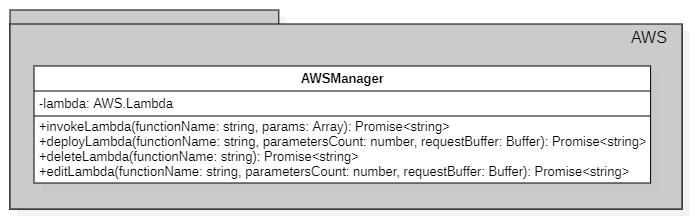
\includegraphics[width=0.8\linewidth]{diagrammi/etherless-server/AWS}
		\caption{Class diagram of the AWS$_{G}$ package.}
	\end{figure}
	\subsubsubsection{AWSManager}
	Class used to communicate with AWS$_{G}$ Services, particularly with AWS Lambda$_{G}$.
	\subsubsubsection*{Attributes}
	\begin{itemize}
		\item \textbf{lambda}: service interface object used to interact with the AWS Lambda$_{G}$ service.
	\end{itemize}
	\subsubsubsection*{Methods}
	\begin{itemize}
		\item \textbf{invokeLambda}: invokes a Lambda$_{G}$ function using the given function name and parameters, returning an asynchronous response or an error message;
		\item \textbf{deployLambda}: invokes the AWSDeployer Lambda$_{G}$ function using the name, the number of parameters and the content of the Lambda$_{G}$ function to be deployed, returning an asynchronous success or error response;
		\item \textbf{editLambda}: invokes the AWSDeployer Lambda$_{G}$ function using the name, the number of parameters and the new content of the Lambda$_{G}$ function to be edited, returning an asynchronous success or error response;
		\item \textbf{deleteLambda}: deletes an existing Lambda$_{G}$ function identified by the given function name, returning an asynchronous success or error response.
	\end{itemize}
	\subsubsection{IPFS}
	This package is used to communicate with the IPFS$_{G}$ service.
	\begin{figure} [h!]
		\centering
		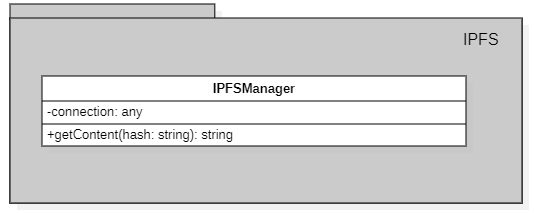
\includegraphics[width=0.8\linewidth]{diagrammi/etherless-server/IPFS}
		\caption{Class diagram of the IPFS$_{G}$ package.}
	\end{figure}
	\subsubsubsection{IPFSManager}
	Class used to communicate with the IPFS$_{G}$ service, specifically to retrieve functions' data in string format. To establish a connection with the IPFS$_{G}$ network we use \texttt{ipfs-mini} API$_{G}$. 
	\subsubsubsection*{Attributes}
	\begin{itemize}
		\item \textbf{ipfs}: object through which the class can interact with the \texttt{ipfs-mini} API$_{G}$.
	\end{itemize}
	\subsubsubsection*{Methods}
	\begin{itemize}
		\item \textbf{getFileContent}: used to retrieve functions' data in string format from IPFS$_{G}$.
		\item \textbf{saveOnIpfs}: used to save data in string format to IPFS$_{G}$.
	\end{itemize}
	\subsubsection{Config}
	This package is used to create and manage configuration objects used by the services that operate inside the system.
	\begin{figure} [h!]
		\centering
		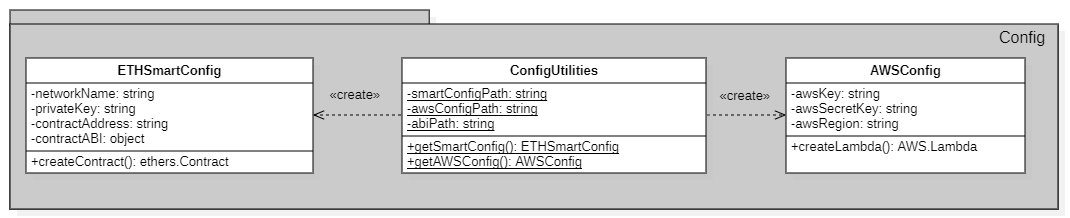
\includegraphics[width=1\linewidth]{diagrammi/etherless-server/Config}
		\caption{Class diagram of the Config package.}
	\end{figure}
	\subsubsubsection{ConfigUtilities}
	Class used to fetch configuration files and to create configuration objects used by services that operate inside the system.
	\subsubsubsection*{Attributes}
	\begin{itemize}
		\item \textbf{smartConfigPath}: string containing the path to the Ethereum configuration file;
		\item \textbf{abiPath}: string containing the path to the abi of the smart contract used for Ethereum communications;
		\item \textbf{awsConfigPath}: string containing the path to the AWS$_{G}$ configuration file.
		\item \textbf{ipfsConfigPath}: string containing the path to the IPFS$_{G}$ configuration file.
	\end{itemize}
	\subsubsubsection*{Methods}
	\begin{itemize}
		\item \textbf{getEthSmartConfig}: returns an ETHSmartConfig object, created using the Ethereum configurations;
		\item \textbf{getAWSConfig}: returns an AWSConfig object, created using the AWS$_{G}$ configurations.
		\item \textbf{getIpfsConfig}: returns an IpfsConfig object, created using the IPFS$_{G}$ configurations.
	\end{itemize}
	\subsubsubsection{EthSmartConfig}
	Class containing the configurations used to communicate with an Ethereum smart contract, allowing the creation of instances of said contract using the Ethers.js$_{G}$ library.
	\subsubsubsection*{Attributes}
	\begin{itemize}
		\item \textbf{networkName}: string containing the name of the Ethereum network to be used for the communication;
		\item \textbf{privateKey}: string containing the private key used to access the Ethereum smart contract;
		\item \textbf{contractAddress}: string containing the address of the Ethereum smart contract.
	\end{itemize}
	\subsubsubsection*{Methods}
	\begin{itemize}
		\item \textbf{createSmartContract}: returns an instance of an Ethereum smart contract created with the configurations contained in the EthSmartConfig.
	\end{itemize}
	\subsubsubsection{AwsConfig}
	Class containing the configurations used to communicate with the AWS$_{G}$, allowing the creation of instances of said services using the aws-sdk library.
	\subsubsubsection*{Attributes}
	\begin{itemize}
		\item \textbf{awsKey}: string containing the key to access the AWS$_{G}$ account used to communicate with AWS$_{G}$;
		\item \textbf{awsSecretKey}: string containing the secret key to access the AWS$_{G}$ account used to communicate with AWS$_{G}$;
		\item \textbf{awsRegion}: string specifying on which region AWS$_{G}$ will operate.
	\end{itemize}
	\subsubsubsection*{Methods}
	\begin{itemize}
		\item \textbf{createLambda}: sets the current AWS$_{G}$ configuration to the ones contained in the AwsConfig object, and returns an instance of a Lambda$_{G}$ service interface object.
	\end{itemize}
	\subsubsection{Lambda}
	This package is a reference to the Lambda$_{G}$ functions the AWS$_{G}$ package interacts with.
	\begin{figure} [h!]
		\centering
		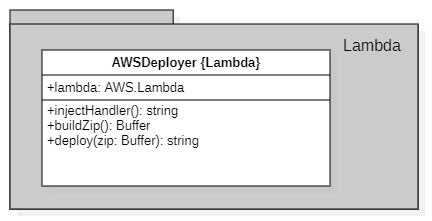
\includegraphics[width=0.7\linewidth]{diagrammi/etherless-server/Lambda}
		\caption{Class diagram of the Lambda$_{G}$ package.}
	\end{figure}
	\subsubsubsection{deployer}
	AWS Lambda$_{G}$ function used to create a handler for the function to be deployed, as well as building a Lambda$_{G}$ deployment package and requesting the deployment itself.
	\subsubsubsection*{Attributes}
	This Lambda$_{G}$ function does not contain any attributes.
	\subsubsubsection*{Methods}
	\begin{itemize}
		\item \textbf{injectHandler}: used to create and inject a handler for the function to be deployed which will be used by Lambda$_{G}$ to handle parameterized invocations to the function;
		\item \textbf{buildZip}: used to build a Lambda$_{G}$ deployment package which consists of a Zip file containing the function to be deployed and all the dependencies required by Lambda$_{G}$;
		\item \textbf{deployFunction}: used to request the deployment of the given Lambda$_{G}$ deployment package to the AWS Lambda$_{G}$ service;
		\item \textbf{editFunction}: used to request the deployment of the given Lambda$_{G}$ deployment package to the AWS Lambda$_{G}$ service, in order to update the code of an existing Lambda$_{G}$ function.
	\end{itemize}
	\newgeometry{a4paper,left=1in,right=1in,top=1in,bottom=1in,nohead}
	\begin{landscape}
	\subsection{UML}
		\begin{figure}[H]
			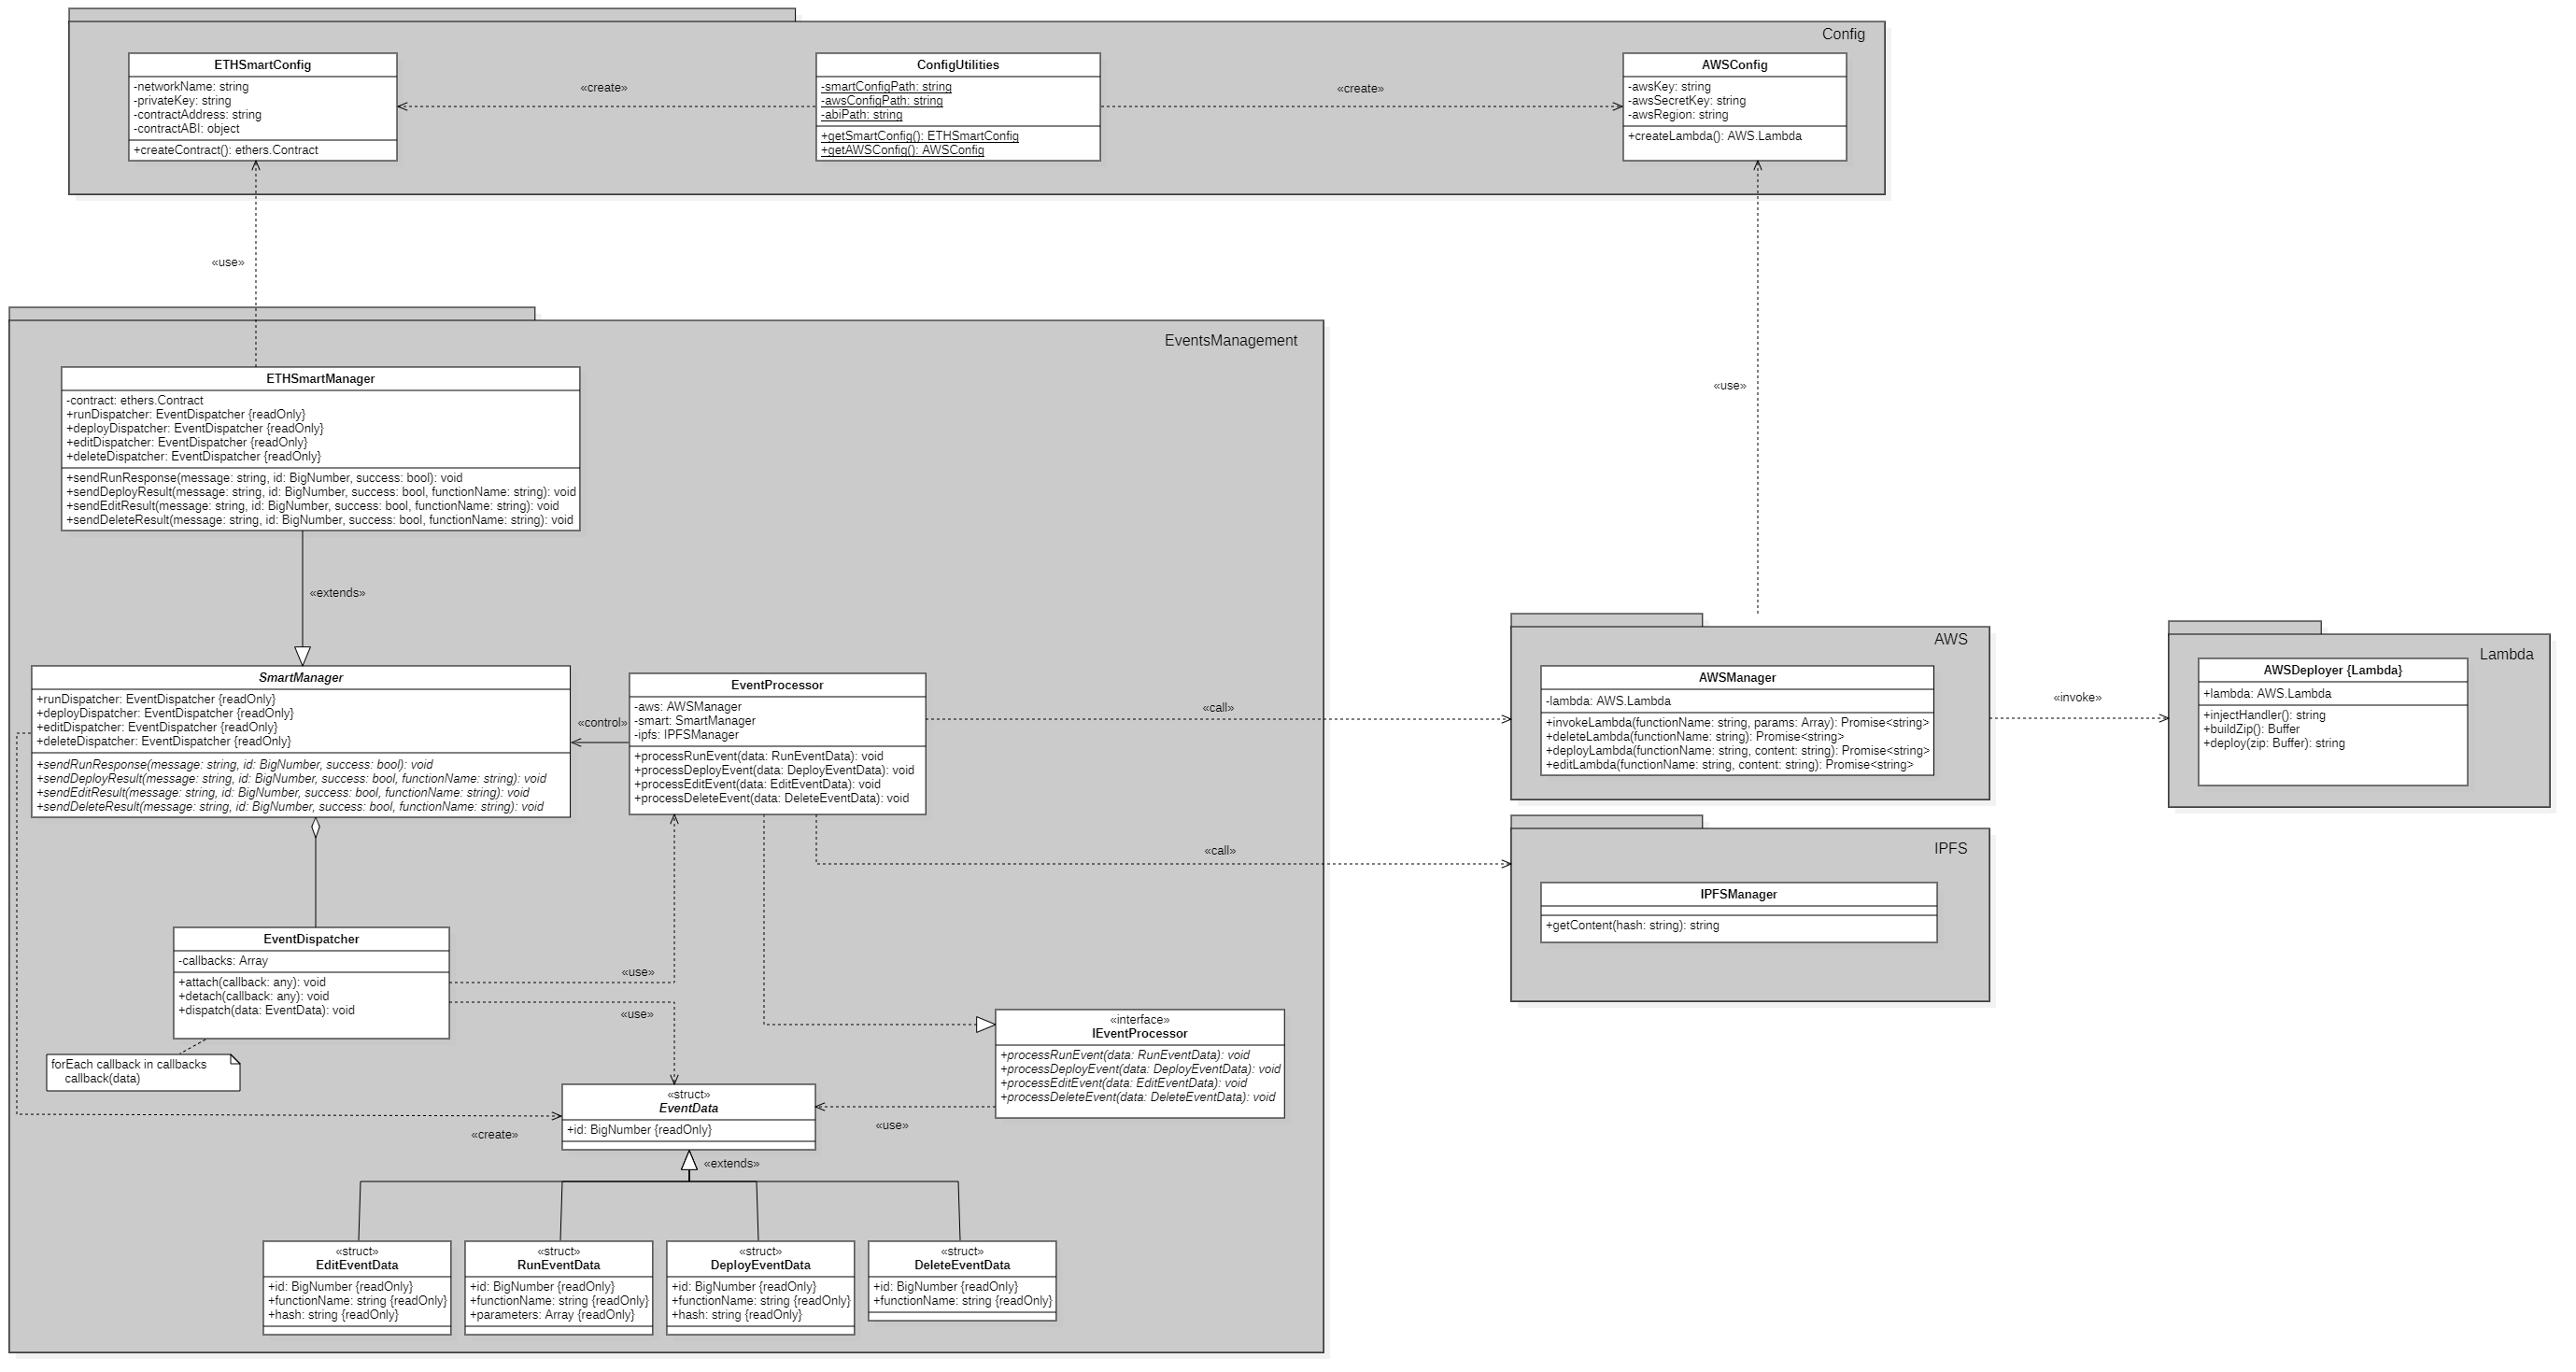
\includegraphics[width=24cm, height=13cm]{././diagrammi/etherless-server/Etherless-server-package-class.png}
			\caption{Etherless-server module architecture.}
		\end{figure}
	\end{landscape}
	\restoregeometry

	\subsection{Extensibility}  %Possibili sviluppi futuri
	The architecture of Etherless-server was designed following the SOLID principles, meaning extensibility is one of its most important characteristics. In order to allow for the integration of new functionalities in the system without heavy alterations of the existing architecture various design choices were implemented.
		\subsubsection{Processing operations}
		The events received from the blockchain are encapsulated into processing requests in the form of EventData objects, which contain the information necessary for the request processing. Specific event dispatchers are then used to forward these objects to all the classes that are interested in the processing of that particular type of request. \\
		This approach allows us to easily introduce new event-processing classes and instances without the need to make any changes to the existing implementation. In fact, in order to receive the processing requests, a newly added class would simply need to subscribe to the event dispatchers that forward the type of requests it is interested to process. \\
		As a consequence, this implementation allows us to develop classes which process only a subset of the processing requests. To achieve this we make use of the Setter Injection design pattern, creating weak dependencies between the events-receiving and the events-processing instances.
		\subsubsection{Event sources}
		The development of SmartManager as an abstract class implies the possibility of handling new types of external events, i.e. events emitted by another blockchain, by creating a new specific derived class. Adding a new type of SmartManager class does not require making any changes to the existing implementation.
		\subsubsection{Event processing}
		The development of IEventProcessor as an interface implies the possibility of introducing new types of processors for the requests, which may handle the requests differently from the existing one. Adding a new type of event-processing class does not require making any changes to the existing implementation.
		\subsubsection{Facade}
		The use of the Facade structural design pattern for the development of the EventProcessor class allows the introduction of new services to be managed by said class. The configuration of the newly introduced services may be handled with an upgrade of the ConfigUtilities class.
		\subsubsection{Processing requests}
		The development of EventData as an abstract class implies the possibility of handling new types of processing requests by creating a new specific derived class.
